\documentclass[11pt]{article}
\usepackage{macros}
\usepackage{bbm}
\usepackage{longtable}
\usepackage{titlesec}


\titleformat{\section}
  {\normalfont\sffamily\Large\bfseries}
  {\thesection}{1em}{}
\titleformat{\subsection}
  {\normalfont\sffamily\large\bfseries}
  {\thesubsection}{1em}{}
  
\titleformat{\subsubsection}
  {\normalfont\sffamily\normalsize\bfseries}
  {\thesubsubsection}{1em}{}
  
\hypersetup{urlcolor=Purple}

% \singlespacing
\newgeometry{left=1in, right=1in, bottom=1.3in}
\title{\sffamily\bfseries{Prediction of the 2018 Midterm Elections}}
\author{Jiafeng Chen\thanks{Harvard College, \url{jiafengchen@college.harvard.edu}} \and Joon Hyuk Yang\thanks{Harvard College, \url{joonhyukyang@college.harvard.edu}}}
\begin{document}
\maketitle
\section{Introduction}

We present a statistical model and a machine learning method to perform
prediction for the 2018 elections of the U.S. House of Representatives. The main
challenge of such a prediction problem is that the historical panel of election
data is short---both in terms of years with adequate non-missing covariates 
(2010--2016) and in terms of observations (435 per year). The shortness in years
creates a generalization problem. All elections in 2010--2016 are considered
Republican wave elections, and models may reasonably display favor towards
Republicans. This problem could be mitigated if we condition on more and more
data and avoid overfitting. However, the low number of observations becomes
extremely problematic, as $p > N$ problems are quickly encountered---especially
with complex basis transforms over the data. Furthermore, the changing political
landscape of 2018 makes real-time polling data quite valuable, but with the lack
of historical polling data, we cannot simply incorporate polling as an
additional feature.

We devise a Bayesian approach that seeks to mitigate these problems. In our
approach, the training data (data before 2018) is used to construct a prior for
2018, which is then updated with polling data for 2018. Our model resembles
what Nate Silver describes FiveThirtyEight's Classic House Forecast Model to
be, where our prior estimation is akin to Silver's ``fundamentals'' and our
polling updating is akin to that in Silver's model. Our approach is fully
compatible with additional features or polls, and admits a few extensions.
Moreover, thanks to a few simplifying approximations we make, our approach is
extremely computationally tractable, while remaining statistically faithful. 

This report is organized as follows. \Cref{sec:data} discusses various datasets
we use and preprocessing applied. \Cref{sec:model} discusses our statistical
model and machine learning method, including parameterizations, estimation
strategies and the considerations therein. \Cref{sec:results} displays various
updated predictions and provides a brief discussion of potential shortcomings
and alternative strategies. \Cref{sec:conc} concludes.

\section{Data}
\label{sec:data}
\subsection{Informative Prior Features}
We first consider a range of potentially relevant features to uncover an overall trend in Midterm Election results since 2010. We collect, process, then use a second-order polynomial basis transform on the features to discover nonlinear correlations in constructing our prior. The following features were used to inform our prior: Republican or Democratic incumbency, gender, voting pattern in the previous presidential election, percentage of minorities, presidential approval rating, candidates’ party alignment with the incumbent president, log of median income, percentage of district population with a Bachelor’s degree or above, one-hot encoding of each state, and the ratio of search frequency via Google Trends.

One design choice we made in feature selection is to ignore Third-party candidates. Since 2010, there was a single Independent candidate (Jo Ann Emerson) who won a seat at the House, and given that there was no evidence to support a sudden surge in Third-party candidates in the 2018 election, we focus on the major parties.

To illustrate the relative importance of these featurees, \Cref{fig:feature} shows the top 10
features in terms of absolute value of weight coefficients. Empirically, we observe that minority percentage, percentage with Bachelor's degree, and presidential approval rating are features that carry the most weight. Note that \textit{rep\_to\_tot\_oct} and \textit{rep\_to\_tot\_nov} also exhibit strong predictive power, each representing the query frequency on Google Trends for the Republican candidate over both candidates in the first half of October and second half of October, respectively.

\subsection{Google Trends}
Google Trends, unlike Google Keyword Planner, shows the \textit{relative} popularity of search queries from a scale of 0 to 100. Relative popularity refers to the ratio of a query's search volumne to the sum of the search volumes of all possible queries. This allows for an easier and more intuitive comparison between terms via search across arbitrary periods of time. Moreover, Google Trends allows for a State-level (but not District-level) granularity in search query trends. We take advantage of this to compare how often a candidate's name was searched in within the State compared to his or her opponent for the first half of October versus the second half of October.

There are two considerations with respect to using Google Trends data. One
obvious but important point to note is that we do not discern the positivity or
negativity of these queries. Instead, we simply observe the total number of
queries. Though this may be a noisy estimate of the true support for a
candidate, as was the case for the 2016 Presidential Election, we adhere to the
notion that \textit{there is no such thing as bad publicity} and The Economist's
article that Google Trends ``provide real-time information that is not available
anywhere else". \footnote{See this
\href{https://www.economist.com/graphic-detail/2016/03/01/how-useful-is-google-search-data-when-predicting-primary-elections}{Economist} article.} Second, the usage of Google as a way to collect information in 2018 increased significantly compared to previous years. Furthermore, the use of Google is biased in favor of a younger population, and may be a disproportionate representation of interest for candidates. With these two caveats in mind, however, we find that the inclusion of Google Trends data augments the information of our prior significantly, compared to a prediction without it.

\subsection{Preprocessing}

In addition to the standard zero-mean and normalization procedure, we employed several techniques to filter, augment, and otherwise preprocess the collected data in order to produce a sensible outcome by making the most out of the data. In the case of gender, the feature set provided by the class was incomplete. In order to fill the NaN values, we use the gender-guesser library to help classify entries in which we lack the information. \footnote{\href{https://pypi.org/project/gender-guesser/}{gender-guesser} Python Library} In the case of a gender neutral names that were not classified in the training data, we populated them with 0.5.

Another feature with a significant number of missing entries was the percentage of self-identifying Republicans versus Democrats in the district. In order to fill the missing entries with a reasonable approximation, we augmented the features with the 2016 State-level political allegiance data if no data was available for the district for any years, while fitting a forward-filling certain years in question for districts that have the data for some years but not others.

For other features with a few NaN values, we made weak assumptions about the similarity of districts within a given year and used neighboring districts' mean to fill the empty entries. 

\subsection{Polling Data for Posterior Updates}
Once we constructed our preliminary model, we collect and utilize two kinds of polling data to update our prior: the generic ballot poll and a district-wide poll. Both the generic and district polling data were collected from FiveThirtyEight. The first is the generic polling data. FiveThirtyEight claims to use a slow moving generic ballot average, incorporating a larger number of polls at the cost of recency of polls.

 \Cref{fig:genpolls} from FiveThirtyEight delineates the estimate by the solid lines while the highlighted badwidth around represents the 90\% confidence interval in which the polls fall. This is determined by a set of factors, including days from poll to election, size of poll, disagreement with other polls, lopsidedness of a race, among others.\footnote{\href{https://fivethirtyeight.com/features/how-the-fivethirtyeight-senate-forecast-model-works/}{How The FiveThirtyEight Senate Forecast Model Works}} The second is the latest district-level polls, also collected by FiveThirtyEight. As we will later discuss in 3.3.2, for both the generic as well as the district poll, we use the a combination of FiveThirtyEight's claimed confidence interval, poll size, and correlated results to estimate in-poll and between-poll variance. Though we have access to metadata such as the simple average error of the polling firm, grading of the quality of the poll, etc. with access to only the most recent polling results for the 2018 Midterm Election, we opt to make use of the provided data that are hold conjugacy properties while being subject to explicit error quantification.

\section{Statistical model and prediction function}
\label{sec:model}
\subsection{Overview}
Let \[Y_i = \frac{\text{Republican}\% }{\text{Republican}\% + \text{Democrat}\%}\] be the proportion of Republican vote share between the major parties in district $i$, where $i$ is indexed by the triple $(\text{state}, \text{district number}, \text{year of the race})$.
%\footnote{Assuming districts have no time dimension: i.e. Alabama-01 is
%represented by different $i,j$'s across two different years. We also assume for
%simplicity that third parties never win elections, which seems accurate in the
%case for 2018.}
Let $x_i\in \R^p$ be a list of features (after suitable basis transformations)
for the district. 

A machine learning method can generate a prediction function $\hat f_{\cal T}$,
where $\mathcal T$ is the collection of $Y_i, x_i$ over the training set.
However, the
distribution of the test set, $Y_i \mid x_i$ for those districts $i$ in 2018 may
be
substantially different from that of $Y_j \mid x_j$ for $j$ in the training
set. Thus $\hat f_{\mathcal T}$ may incur large generalization errors, since we
are attempting to generalize the prediction function to a potentially 
\emph{different}
distribution
of the data.\footnote{Note that this problem is mitigated by increased data
availability---for instance, if we had obtained historical polling data,
which is difficult to obtain---but we incur a different problem ($p > N$) of
high-dimensional
inference in that case.} Fortunately, we have an additional piece of
information, namely polling data, that we may scrape from polling aggregators
like
FiveThirtyEight.\footnote{\url{https://projects.fivethirtyeight.com/polls/}} The
lack of historical polling data means that we cannot simply include them in the
features $x_i$. Therefore, to incorporate polling data, we perform a two-step
Bayesian procedure. In the first step, we estimate a prior $Y \sim p_{\theta_0,
X}$, where parameters $\theta_0$ is estimated from the training data. In the
second step, we assume that polling data, $Z$, comes from some conditional
distribution $Z \mid Y \sim p_{\eta}(z\mid y)$ for some known or
estimated parameters
$\eta$. We form our final prediction by computing the posterior distribution $Y
\mid Z$. We now discuss how we parameterize $p_{\theta, X}$ and $p_\eta$.

\subsection{Parameterizations}

For the prior, $p_{\theta, X}(y)$, we assume a linear probability model,
\begin{equation}
    Y \sim \Norm(\underbrace{X\beta_0}_{\mu_0}, \Sigma_0)
    \label{eq:first_stage}
\end{equation}
\eqref{eq:first_stage} is misspecified since $Y_i \in [0,1]$ but the Normal
distribution is supported on $\R$. A properly specified generalized linear model
for $Y_i$ is a Beta linear model \citep[See][for an overview]{grun2011extended}.
We have a few reasons for preferring \eqref{eq:first_stage} instead. First, we
note that for large values of $a,b$ in $\Beta(a,b)$, the distribution
$\Beta(a,b)$ is approximately Normal. Second, we note that \[Y_i =
\sum_{j=1}^M \frac{\mathbbm{1} (\text{vote}_j \in \{D,R\})}{\sum_{j'=1}^M \mathbbm{1}
(\text{vote}_{j'} \in \{D,R\})} \mathbbm{1}(\text{vote}_j = R),\] for a district with
$M$ voters, which should have an approximately Normal distribution, by the
Central Limit Theorem. Third, computational methods for the Beta regression
model---especially those that deal effectively with high-dimensional
covariates---is much less readily available than those for the Normal linear
model. We note additionally in \Cref{fig:qq} that the fitted residuals are
approximately Normally distributed and in \Cref{fig:diag} that they are homoskedastic, and we note that Normal distribution eases
computation for Bayesian updating in our next step. For \eqref{eq:first_stage},
we need to estimate $\theta_0 = (\beta_0, \Sigma_0)$. 

For $p_{\eta}$, we assume that conditional on $Y$, the polls $Z_j$ are
independently distributed. We can treat an observation of a poll $z_j$ as
generated by
asking $n_j$
individuals a question (``Are you voting for the Republican candidate''), with
$z_j \in [0,1]$ respondents responding
affirmatively.\footnote{Again, this model assumes that the only parties running
are Republicans and Democrats, and that there are no undecided individuals.
When working with data, we normalize the Republican percentage by the sum of
the Republican and Democratic percentages.}
Assume that 
\begin{equation}
    Z_j \mid Y \sim \Norm(a_j^T Y, \sigma_{Z_j}^2), \text{ for $a_j, \sigma_
    {Z_j}^2$ that do not depend on $Y$}.
    \label{eq:polls}
\end{equation}
We use the Normal distribution in \eqref{eq:polls} because (1) The Normal
distribution works well computationally with our Normal prior\footnote{This is
assuming that the Normal likelihood has variance unaffected by the
prior---which requires a further justification that we discuss in 
\Cref{sec:estimate}.} and (2) polling proportions are empirical averages, which
tend to be Normally distributed by the Central Limit Theorem.



We use two types of polls in our implementation. First is a national
\emph{generic ballot} poll, which simply asks the respondent which party she
would vote for. For such $Z_j$, we assume $a_j = n^{-1} \bm 1$, treating the
mean of such a poll as aggregated over all contested districts. Second is a
district-wide poll, and we use $a_j = e_i$ for a poll in district $i$, where
$e_i$ is the $i$-th standard basis vector. For \eqref{eq:polls}, we need to
estimate $\sigma_{Z_j}^2$ for both types of polls.

We now discuss our approaches to estimation and justify discretionary choices
made therein. 

\subsection{Estimation}
\label{sec:estimate}
\subsubsection{Estimation for $\theta_0$}
We first discuss estimation for $\theta_0 = (\beta_0, \Sigma_0)$.
Let \begin{equation}
\hat \beta_0 = \argmin_\beta \, \sum_{i=1}^{|\mathcal T|} w_i (y_i - x_i^T
\beta)^2
+ \lambda
\pr{\alpha \norm{\beta}_1 + (1-\alpha) \norm{\beta}_2^2}
\tag{Estimation for $\beta_0$}
\label{eq:beta}
\end{equation}
be fitted with an elastic net regularizer over the training data with weights
$w_i$,
where
$(\alpha, \lambda)$ is chosen via 10-fold cross-validation. The weights we chose is uniform $w_i = 1$; however, in the spirit of efficient
estimation as in weighted least
squares, it may be desirable to choose the weights to the proportional to total
votes cast, since we should expect that variance of the measurement $Y_i$ is
inversely proportional to the number of votes cast, as $Y_i$ is an empirical
average. In numerical experimentation, we found that the weights do not affect
results much, and we keep $w_i = 1$ for simplicity.

It is crucial, for the purpose of uncertainty quantification, that we perform good variance estimation. Let $S_i = \{j: \mathsf{state}(j) = 
\mathsf{state}(i)\}$ be those districts in the same state as $i$ (across time),
\[
\hat \Sigma_{ii} = \frac{1}{|S_i|} \sum_{j\in S_i}
\pr{y_j
- x_j^T \hat \beta_0}^2 \tag{Estimation for variance}
\label{eq:var}
\]
be an estimate for variance. Here we estimate variance by pooling over the state
of a district, as states boundaries, unlike district boundaries, do not change
over time. Alternatively, we could estimate variance by letting $S_i$ be those
districts that share the same state and district identifier (which may not be
the same geographical area due to redistricting), or with the $k$ nearest geographical neighbors of district $i$ (in the spirit of $k$NN). 

Optionally, we also estimate off-diagonal elements of $\Sigma$. If district boundaries do not change over time, then we can easily estimate off-diagonal entries of $\Sigma$ as well, since we can use the variation over time to calculate the empirical analogue of covariance: \[
\hat \Sigma_{ij} = \frac{1}{T}\sum_{t=1}^T \pr{y_{it} -x_{it}^T \hat \beta_0}\pr{y_{jt} -x_{jt}^T \hat \beta_0} \tag{Estimation for covariance}
\label{eq:covar}
\]
This approach is no longer valid when district boundaries change over time. Nonetheless, we can still calculate $\hat \Sigma_{ij}$, ignoring district boundary changes.  Note that \eqref{eq:var} is inconsistent with \eqref{eq:covar}, and filling in estimates from \eqref{eq:covar} directly into $\Sigma$ would generate non-positive-definite matrices. As a result, we estimate the \emph{correlation} $\hat \rho_{ij}$ similar to \eqref{eq:covar},\footnote{We fill undefined values of $\hat \rho_{ij}$ with zero.} and use the estimate 
 \[
\hat \Sigma_{ij} = \hat \rho_{ij} \hat \Sigma_{ii} \hat \Sigma_{jj}
 \tag{Estimation for covariance with correlation}
\label{eq:covar_corr}
\]
which ensures that the resulting $\Sigma_0$ is positive definite. \Cref
{fig:hists,fig:diag} displays the Bayesian updating for both specifications,
$\Sigma_0$ diagonal and $\Sigma_0$ fully general. They do not display signifcant
differences.

Now we discuss a few caveats regarding variance estimation. In principle, the variance we estimate should also take into account the uncertainty in $\hat \beta_0$. However, there is little consensus in uncertainty quantification for methods like elastic net and LASSO \citep{kyung2010penalized}, which remains an active research area. The fitting (along with cross-validation) is too expensive to bootstrap either, and we ignore the uncertainty in $\hat \beta_0$ for simplicity. Moreover, \eqref{eq:var} is likely an underestimate of variance---in linear regression, for example, we inflate the naive variance estimate by $n/(n-p)$, where $p$ is the degrees of freedom in a linear regression. The analogous inflation in our setting is with the degree of freedom in the elastic net \citep{zou2007degrees}---the estimate of the degree of freedom is about 100 for a dataset with $N=1500$; thus the inflation factor is about $\frac{1500}{1500-100} \approx 1.07$ for variance, which is sufficiently small to ignore. An alternative would be to estimate variance on a hold-out set, which is unbiased if the data is i.i.d.; we do not hold out for the sake of increasing training data.  

As a notational matter, we now suppress the hat notation on $\beta_0, \Sigma_0.$

\subsubsection{Estimation for polling variance}

We now turn to estimation of variance in the likelihood of polls, $\sigma_{Z_j}^2$ in \Cref{eq:polls}. The main problem in variance estimation is to account for the large between-poll variance unpredicted by a simple model. Suppose poll outcomes are indepedently $n_j^{-1} \Bin(n_j, Y_i)$ conditional on $Y_i$, then the (conditional) standard deviation is as low as $1.58$ percentage points for a poll with $1000$ respondents. However, polls of this size display much more variation than predicted by a simple independent Binomial model. Therefore, we assume that there is some structural between-poll variance and attempt to estimate it from data.  

For both types of polls, there is a within poll variance generated by sampling, and a between-poll variance. The within poll variance is $n_j^{-1}\E[Z_j \mid Y](1-\E[Z_j\mid Y]) \le (4n_j)^{-1}$, which in general depends on $Y$. For computational simplicity, we use the upper bound $\frac{1}{4n_j}$ as a proxy for the within-poll part of variance, since it does not depend on $Y_i$ in order to take advantage of Bayesian conjugacy; the approximation is good for districts with $Y_i$ close to $1/2$, which is precisely those polls that we especially care about. Full, proper posterior condition can still be achieved if we use the more precise estimate, $Y_i(1-Y_i)/n_j$, via an MCMC sampler. 

For a generic ballot poll $Z_j$, we leverage the \href{https://projects.fivethirtyeight.com/congress-generic-ballot-polls/}{FiveThirtyEight polling average estimates} since FiveThirtyEight provides a 90\% confidence interval. We use the (most recent) variance that implies the range of $90\%$ confidence computed by FiveThirtyEight. The FiveThirtyEight estimates are via kernel-weighted local polynomial smoothing,\footnote{The link on footnote 2 in \href{https://fivethirtyeight.com/features/heres-a-new-less-volatile-version-of-our-generic-ballot-tracker/}{FiveThirtyEight's methodology} links to the Stata manual for kernel-weighted local polynomial smoothing.} whose confidence comes from (we conjecture) bootstrapping. We directly use FiveThirtyEight's estimates, as the between-poll part of the variance for generic-ballot polls, for convenience. 

For a district-wide polls $Z_j^i, j = 1,\ldots,J_i$, the variance comes from two components. The first component comes from the sampling error of the poll itself, which is the Binomial variance $\frac{Y_i(1-Y_i)}{n_j} \le \frac{1}{4n_j}$. The second component comes from a between-poll variance, which we estimate by taking the empirical variance of poll results in a district.\footnote{Filling missing values with state-averages.} 

To summarize, we use \begin{align*}
\sigma^2_{Z_j} &= \frac{1}{4n_j} + \sigma^2_{538} \tag{Estimation for generic ballot poll variance}\\
\sigma^2_{Z_j} &= \frac{1}{4n_j} + \hat\sigma^2_{i,p} \tag{Estimation for district poll variance}
\end{align*}
where $ \sigma^2_{538}$ is the variance implied by FiveThirtyEight's 90\% confidence interval, and $\hat \sigma_{i,p}^2$ is the variance of polling results for district $i$ estimated by taking the empirical variance within district $i$.

\subsection{Putting it all together: updating prior}
From estimating $\theta_0$, for the competitive races in 2018, we obtain a prior estimate $Y \sim \Norm(\mu_0, \Sigma_0)$, where $\mu_0 = X\beta_0$. The polls form a vector $Z \mid Y \sim \Norm(\mu_Z, \Sigma_Z)$ for $\mu_Z, \Sigma_Z$ compatible with our assumptions. Therefore, our posterior is \[
Y\mid Z \sim \Norm\pr{(\Sigma_0 + \Sigma_Z)^{-1} \pr{\Sigma_Z\mu_0 + \Sigma_0 \mu_Z}, \pr{\Sigma_Z^{-1} + \Sigma_0^{-1}}^{-1}}.
\]

Prediction for a single district simply takes the entry corresponding to the
district in the distribution $Y \mid Z$, a marginally Normal distribution, and
computes the probability that the Normal random variable is greater than $0.5$,
which is equal to the (marginal) probability that a Republican wins in the
district. Prediction for the entire race (as in 
\Cref{fig:hists,fig:diagonal_prior,fig:hists_diffuse}) is done by drawing
$\tilde y$ from $Y \mid Z$ and computing the number of entries for which
$\tilde y_j > 0.5$, as the seats that Republicans win among the competitive
seats.

% Let $\hat \sigma_{0i}^2 = \sum (y_j - x_j^T \hat\beta_0)^2$ be fitted as the variance of the residuals, where the sum could be over districts in the same state, over all districts, or some kernel-weighted estimator. For simplicity, we stratify variance estimate by state.\footnote{One could also estimate variance over a holdout set, which might improve bias.} Let $\hat \mu_{i0} = x_i^T \hat \beta_0$.


% For a district that corresponds to an upcoming election, we form a prior 
% $Y_i\sim \Norm(\hat \mu_{i0}, \hat \sigma_0^2),$ or in vector form \[
% Y \sim \Norm(\hat \mu_0, \hat \Sigma_0)
% \]
% Note that in such a formulation, we ignore the sampling variance of $\hat
% \mu_{i0}$ and $\hat \sigma_0^2$,\footnote{The elastic net regularizer in the
% fitting method for $\beta$ makes the sampling variance of $\hat\beta_0$
% difficult to compute.} instead forming a plug-in estimate, appealing to the law
% of large numbers.\footnote{From this point on, we drop the hat on $\mu_{i0},
% \sigma_0$.} To obtain a more accurate and timely prediction for the district, we
% update the prior in two steps.

% First, to take into account the ``blue wave,'' we update our prior via the generic congressional ballot.\footnote{\url{https://projects.fivethirtyeight.com/congress-generic-ballot-polls/}} Formally, we model generic congressional poll as $Z_{G} \mid Y_i \sim \Norm(Y_i, \sigma_G^2),$ where $\sigma_G^2$ is estimated from the 90\% confidence interval provided by FiveThirtyEight. We have the following data generating process: \begin{align*}
% Y &\sim \Norm(\hat \mu_0, \hat \Sigma_0)\\
% Z_G \mid Y &\sim \Norm\pr{n^{-1}1^T Y, \sigma_G^2}
% \end{align*}

% We update our prior to form an intermediate posterior: \[
% Y \mid Z_G \sim \Norm(\mu_1, \Sigma_1).
% \]
% From now on, we drop the conditioning on $Z_G$.

% Second, for some districts, we observe a number of district-specific polls $Z_{i1},\ldots,Z_{iJ_i}$.\footnote{In practice, we take the $J$ most recent polls (if available) in district $i$, where $J = 10$.} The variance across polls is much higher than implied by a simple Beta-Binomial model, where one assumes that each poll is an independent $\Bin(n_j,p)$ where $p$ is sampled from a Beta (again, approximately Normal) prior. As such, we hesitate from using a simple Beta-Binomial updating procedure and opt for the following model: We assume that poll $j$ has an independent bias $\epsilon_j \sim \Norm(0, \sigma^2_p)$, where $\sigma_p$ is estimated as the empirical variance of poll outcomes in a district: \begin{align*}
% Y &\sim \Norm(\mu_1, \Sigma_1) \quad \epsilon_j \sim \Norm(0, \sigma_p^2) \\
% Z_{ij}\mid Y_i, \epsilon_j &\sim n^{-1} \cdot \Bin(n, e_i^T Y + \epsilon_j),
% \end{align*}
% where $e_i$ is the $i$th standard basis vector. It's somewhat difficult to compute the posterior $Y \mid Z_{i1}, \ldots, Z_{iJ}$. Instead we may assume the misspecified model, justified as $n^{-1}\Bin(n, p)$ is approximately Normal when $n$ is large. \begin{align*}
% Y &\sim \Norm(\mu_{1}, \Sigma_{1}) \\
% Z_{ij} \mid Y &\sim \Norm\pr{e_i^TY, \frac{1}{4n_j} + \sigma_p^2},
% \end{align*}
% so as to (a) take advantage of Normal-Normal conjugacy and (b) ignore the dependence of $\var(Z_{ij})$ on $Y_i$. We now have the posterior by, say, sequentially Bayesian updating: \[
% Y \mid (Z_{i1},\ldots,Z_{iJ_i})_{i=1}^n \sim \Norm\pr{
%     \mu_{2}, \Sigma_{2}
% }.
% \]
% We predict $\hat Y_i = \mu_{2i}$, and, naturally \[
% \hat{\text{Winner}}_i = \begin{cases}
%     \text{Republican} & \mu_{2i} > .5 \\
%     \text{Democrat} & \mu_{2i} < .5
% \end{cases}
% \]

\section{Results}
\label{sec:results}
\subsection{Testing the Normality Assumption}
Before discussing the outcome of our prediction, we first verify our initial assumption that the underlying distribution is, in fact, Normal. We do so by plotting the following Q-Q plot. Indeed, through a quick visual inspection of \Cref{fig:qq}, the empirical quantile and the true Normal quantile form a roughly straight line, suggesting our assumptions hold water.

Next, we examine the residuals and the fitted value regressing over them. \Cref{fig:diag} shows that the residuals are approximately centered around 0, and combined with \Cref{fig:qq}, we observe that their spread is also approximately normal and homoskedastic.

\subsection{Final Projection and Baseline Comparisons}
Our final prediction for the 2018 Midterm Elections is shown in \Cref{fig:hists}. We observe the empirical distributions of our prior, posterior after updating with the generic ballot, and the final posterior after updating with the district-level polls from section 3.4.

As discussed in sections 2 and 3, our prior is informed by the collected historical data. Reflecting the ground truth trend of Republican dominance in the House, our prior is centered at a Republican majority with the likelihood of Democrats taking the majority at 17\%. With subsequent polling updates to our prior, we observe the posterior shift to a Democratic majority with a slightly higher peak. 

Our final posterior presented in \Cref{fig:hists} makes use of $\Sigma_0$ for our prior covariance matrix where the off-diagonal entries are estimated via the empirical variation over time assuming unchanged district boundaries. If we assume independence across each district, we have a diagonal $\Sigma_0$, which produces the result of \Cref{fig:diagonal_prior}. A quick visual inspection shows that posterior is centered slightly more conservatively, giving the Democrats a slightly smaller margin of victory (86\% chance of winning the majority after the generic ballot update, and 94\% after the district poll update).

To illustrate the informative nature of our data-derived prior, we plot the shift in distribution with an uninformed prior $\Norm(0.5\bm{1}, 10I)$ in \Cref{fig:hists_diffuse}.

\Cref{fig:538_hist} provides FiveThirtyEight's predictions on the day before the Election as a baseline against which we can compare our own predictions. Note the wider tails in FiveThirtyEight's prediction and a more favorable mean for the Democrats than our predictions.

As a final comparison against FiveThirtyEight's baseline, we map our prediction on the district level in \Cref{fig:proj_map} and compare our results against that of FiveThirtyEight in \Cref{fig:538_map}.

\section{Conclusion, Discussion, and Future Considerations}
\label{sec:conc} 

Our results show that the Democrats will take over the majority in the House after the 2018 Midterm Elections with 94.5\% probability. This posterior comes after our prior trained on our historical data predicts a 17.2\% probability and the first posterior after the generic poll update that predicts a 87.7\% probability of a Democratic House. FiveThirtyEight's prediction, as of November 5, 2018, predicts that the Democrats will take control of the House with an 87.5\% probability.

As is evident, our prediction becomes progressively confident after each additional polling result. This follows from our full posterior \[
Y\mid Z \sim \Norm\pr{(\Sigma_0 + \Sigma_Z)^{-1} \pr{\Sigma_Z\mu_0 + \Sigma_0 \mu_Z}, \pr{\Sigma_Z^{-1} + \Sigma_0^{-1}}^{-1}}\] where both $\Sigma_0$  and $\Sigma_Z$ are positive definite and by our assumption of conditional independence of district polls, $\Sigma_Z$ is diagonal.


\section{Figures}
\label{sec:figures}

\begin{figure}[tbh]
  \centering
  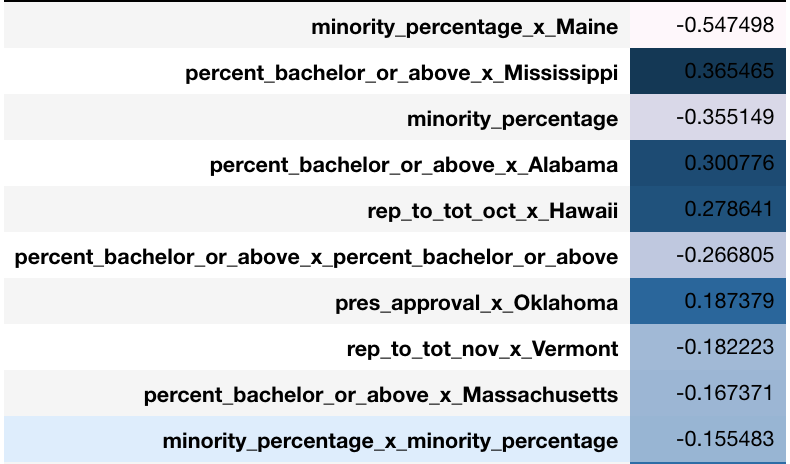
\includegraphics[scale=0.8]{feature_coeff}
  \caption{Some feature coefficients}
  \label{fig:feature}
\end{figure}

 \begin{figure}[tbh]
  \centering
  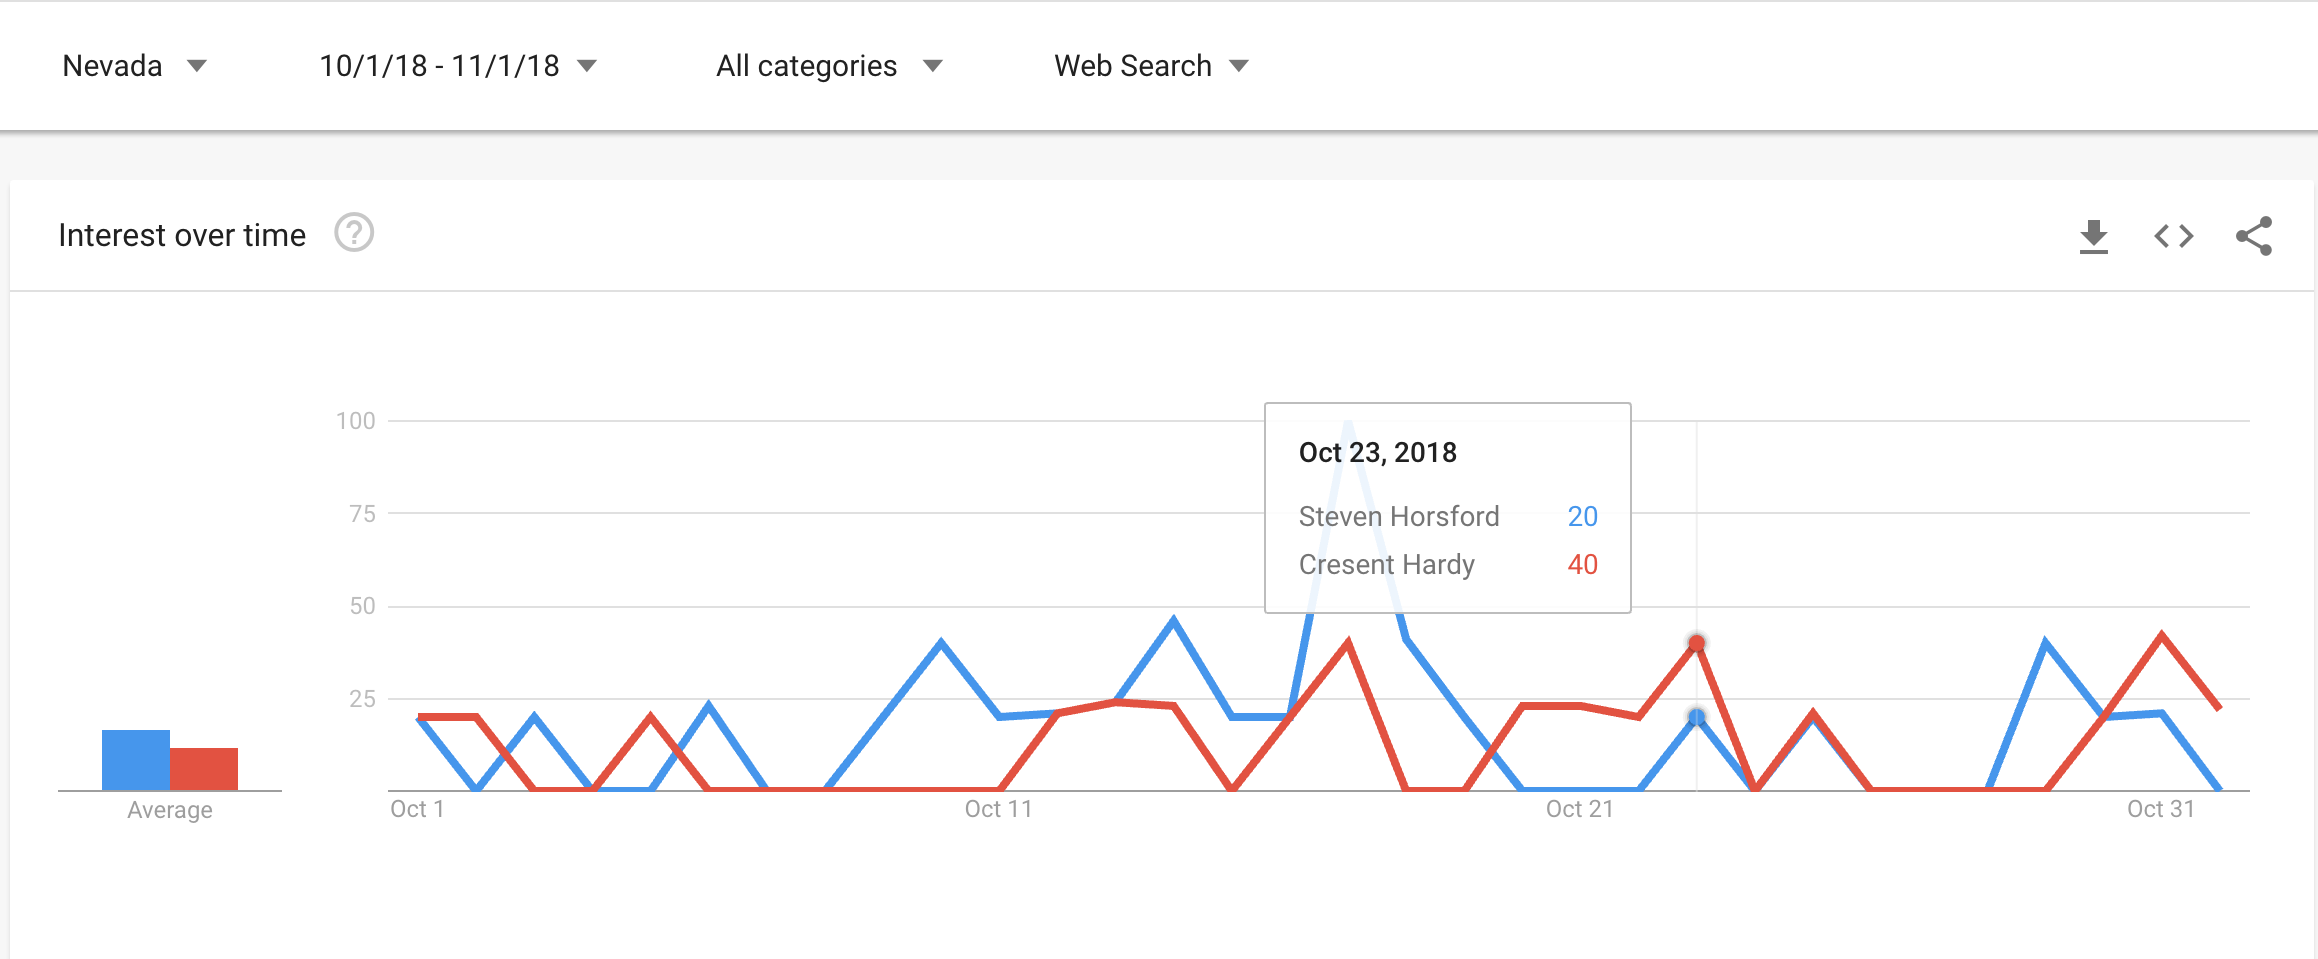
\includegraphics[scale=0.4]{google_trends_ex}
  \caption{Google Trends Nevada District 4}
  \label{fig:trends}
\end{figure}

 \begin{figure}[tbh]
  \centering
  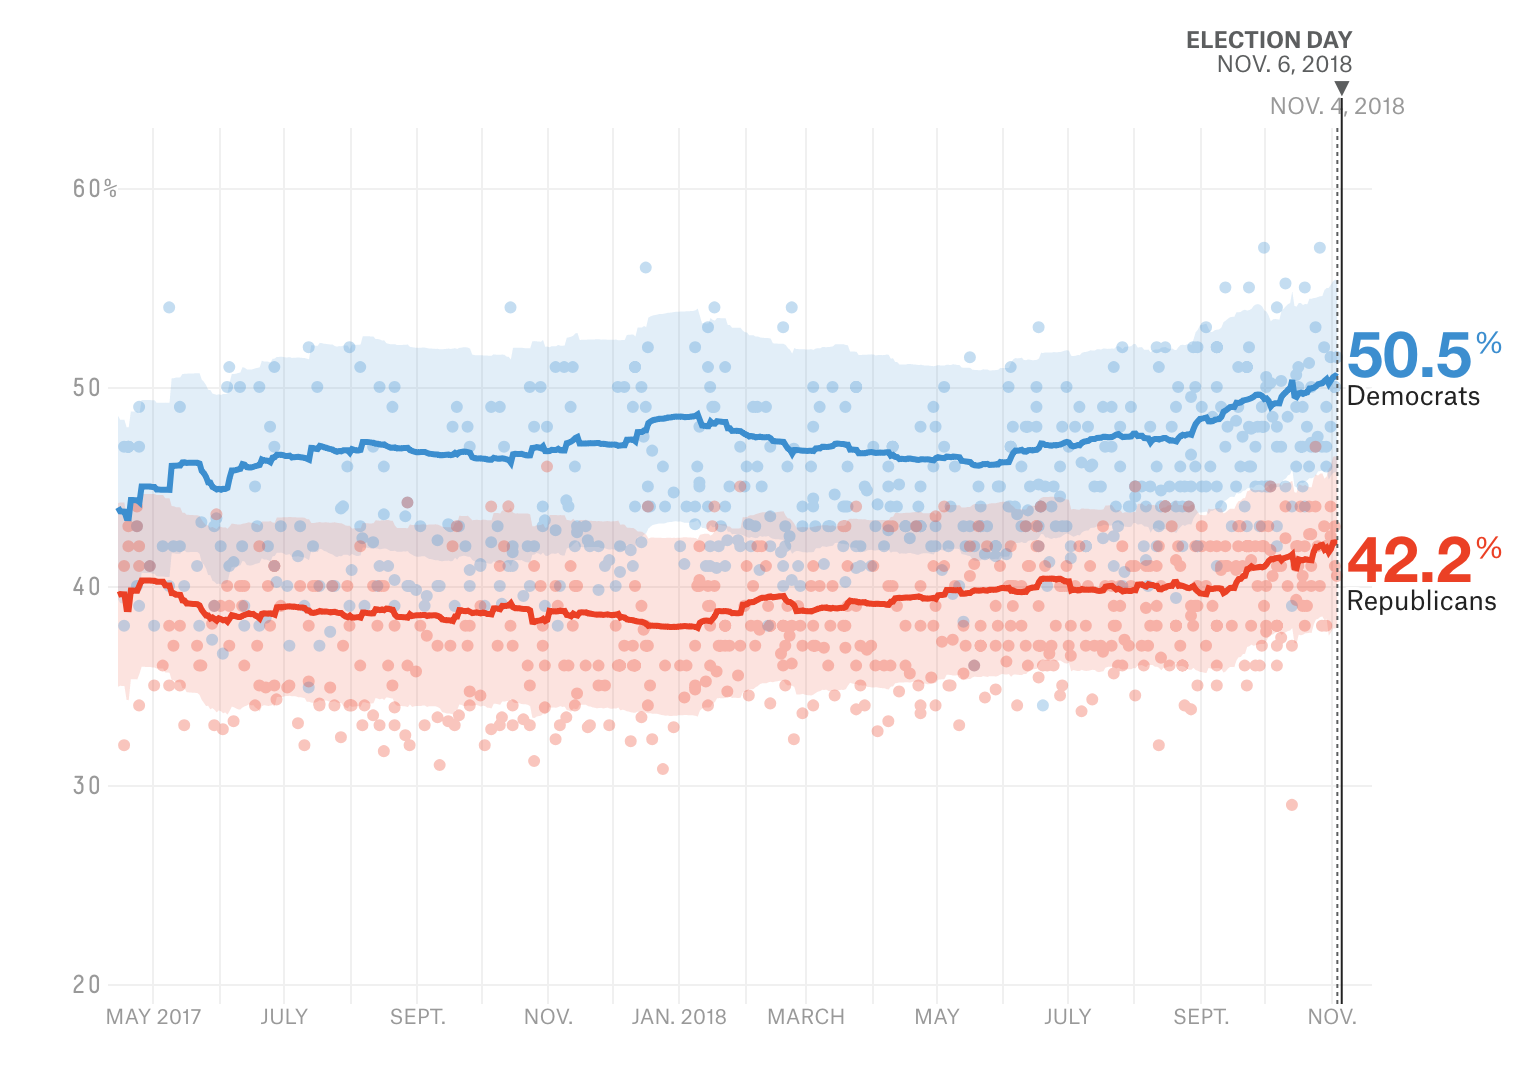
\includegraphics[scale=0.45]{general_polling}
  \caption{FiveThirtyEight General Polling Data}
  \label{fig:genpolls}
\end{figure}

 \begin{figure}[tbh]
  \centering
  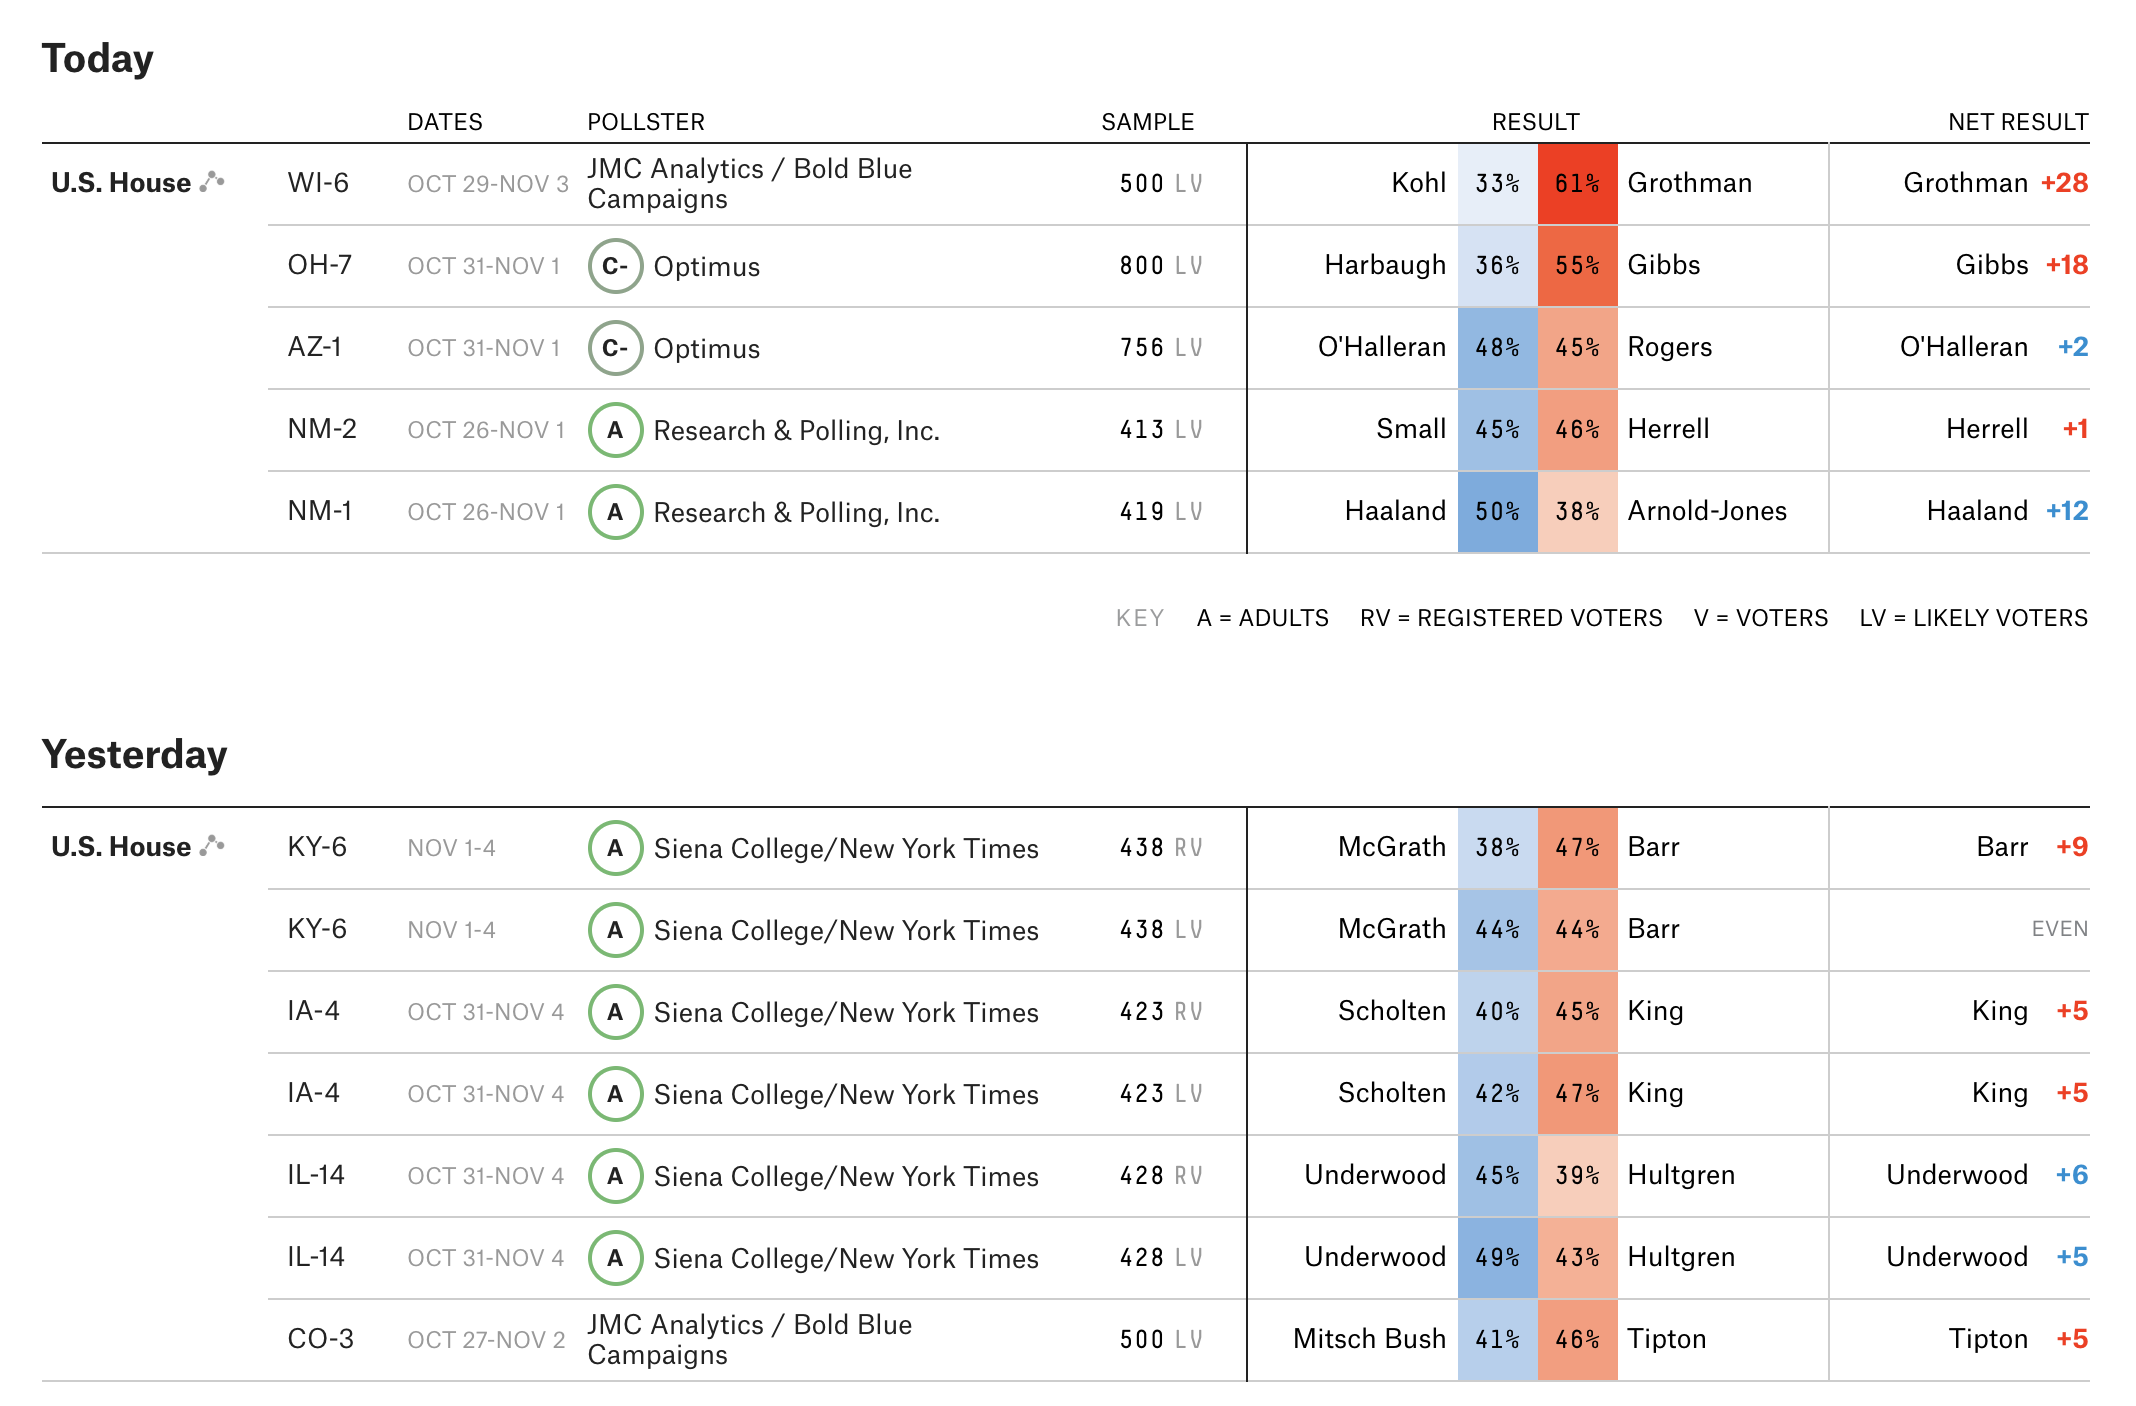
\includegraphics[scale=0.4]{district_polls}
  \caption{FiveThirtyEight District Polling Data}
  \label{fig:distpolls}
\end{figure}

\begin{figure}[tbh]
  \centering
  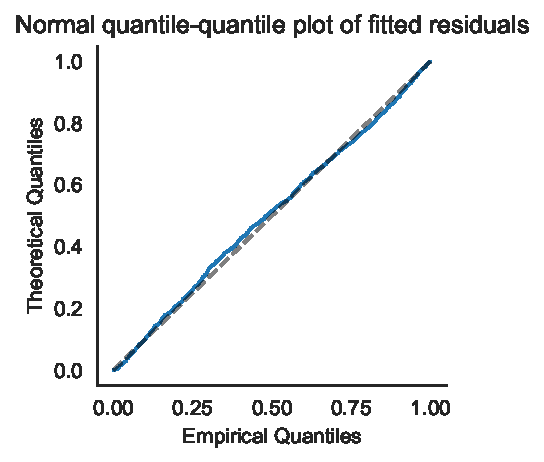
\includegraphics{qq.pdf}
  \caption{Normal Q-Q plot of residuals in fitting \eqref{eq:beta}}
  \label{fig:qq}
\end{figure}

\begin{figure}[tbh]
  \centering
  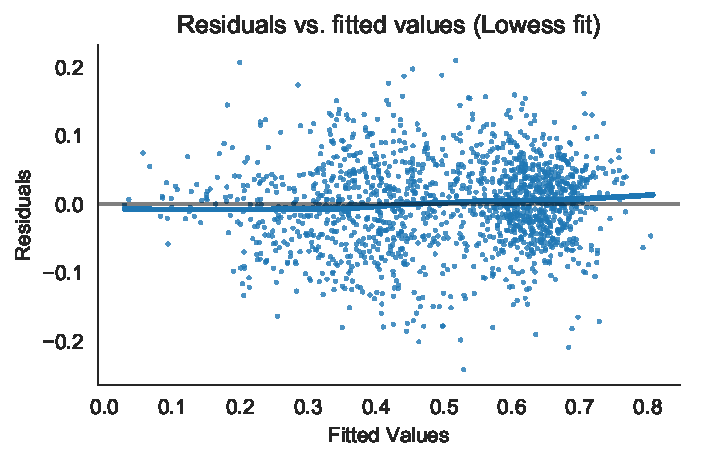
\includegraphics{diagnostics.pdf}
  \caption{Regression diagnostics in fitting \eqref{eq:beta}}
  \label{fig:diag}
\end{figure}

\begin{figure}[tbh]
  \centering
  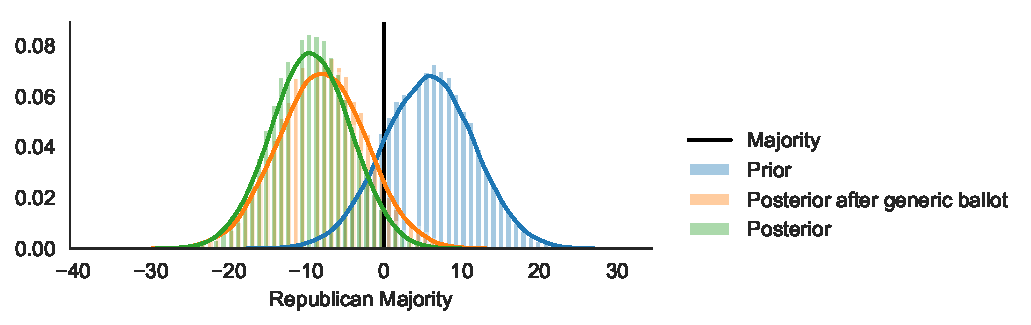
\includegraphics[width=\textwidth]{rep_seats.pdf}
  \caption{Projected Republican seat distribution from prior, intermediate
  posterior, and full posterior with fully general $\Sigma_0$}
  \label{fig:hists}
\end{figure}

\begin{figure}[tbh]
  \centering
  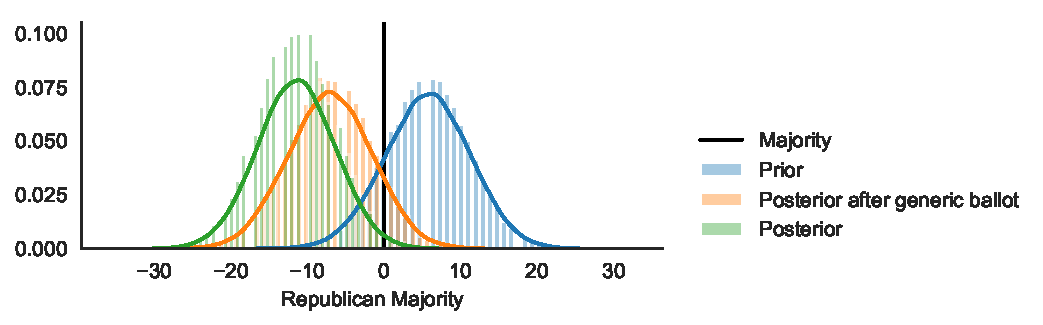
\includegraphics[width=\textwidth]{rep_seats_with_diagonal_prior.pdf}
  \caption{Projected Republican seat distribution from prior, intermediate
  posterior, and full posterior with diagonal $\Sigma_0$}
  \label{fig:diagonal_prior}
\end{figure}

\begin{figure}[tbh]
  \centering
  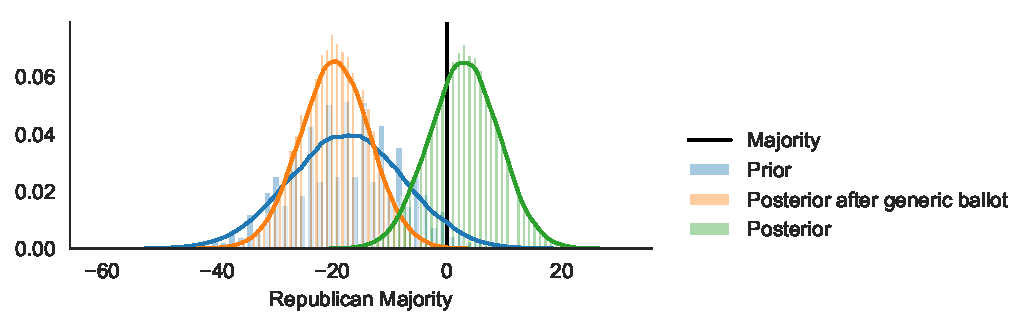
\includegraphics[width=\textwidth]{rep_seats_with_diffused_prior.pdf}
  \caption{Projected Republican seat distribution from prior, intermediate posterior, and full posterior, if we use a $\Norm(0.5\bm{1}, 10I)$ prior for the contested races. It may be odd that the prior is not centered at zero. The reason is that there are more races in which the Democrat is uncontested than those in which the Republican is. It may also be odd that the full posterior shifts the distribution to the right, unlike in \Cref{fig:hists}. The reason is that the district-wide polls shrink variance dramatically, and if the \emph{polled} districts are disproportionately Republican-leaning, then among the districts we are confident about, more districts are Republican-leaning. This would shift the seat distribution to the right, even though more values of posterior mean are less than $0.5$ (Democratic majority), since more Democratic districts have large variance.}
  \label{fig:hists_diffuse}
\end{figure}

\begin{figure}[tbh]
  \centering
  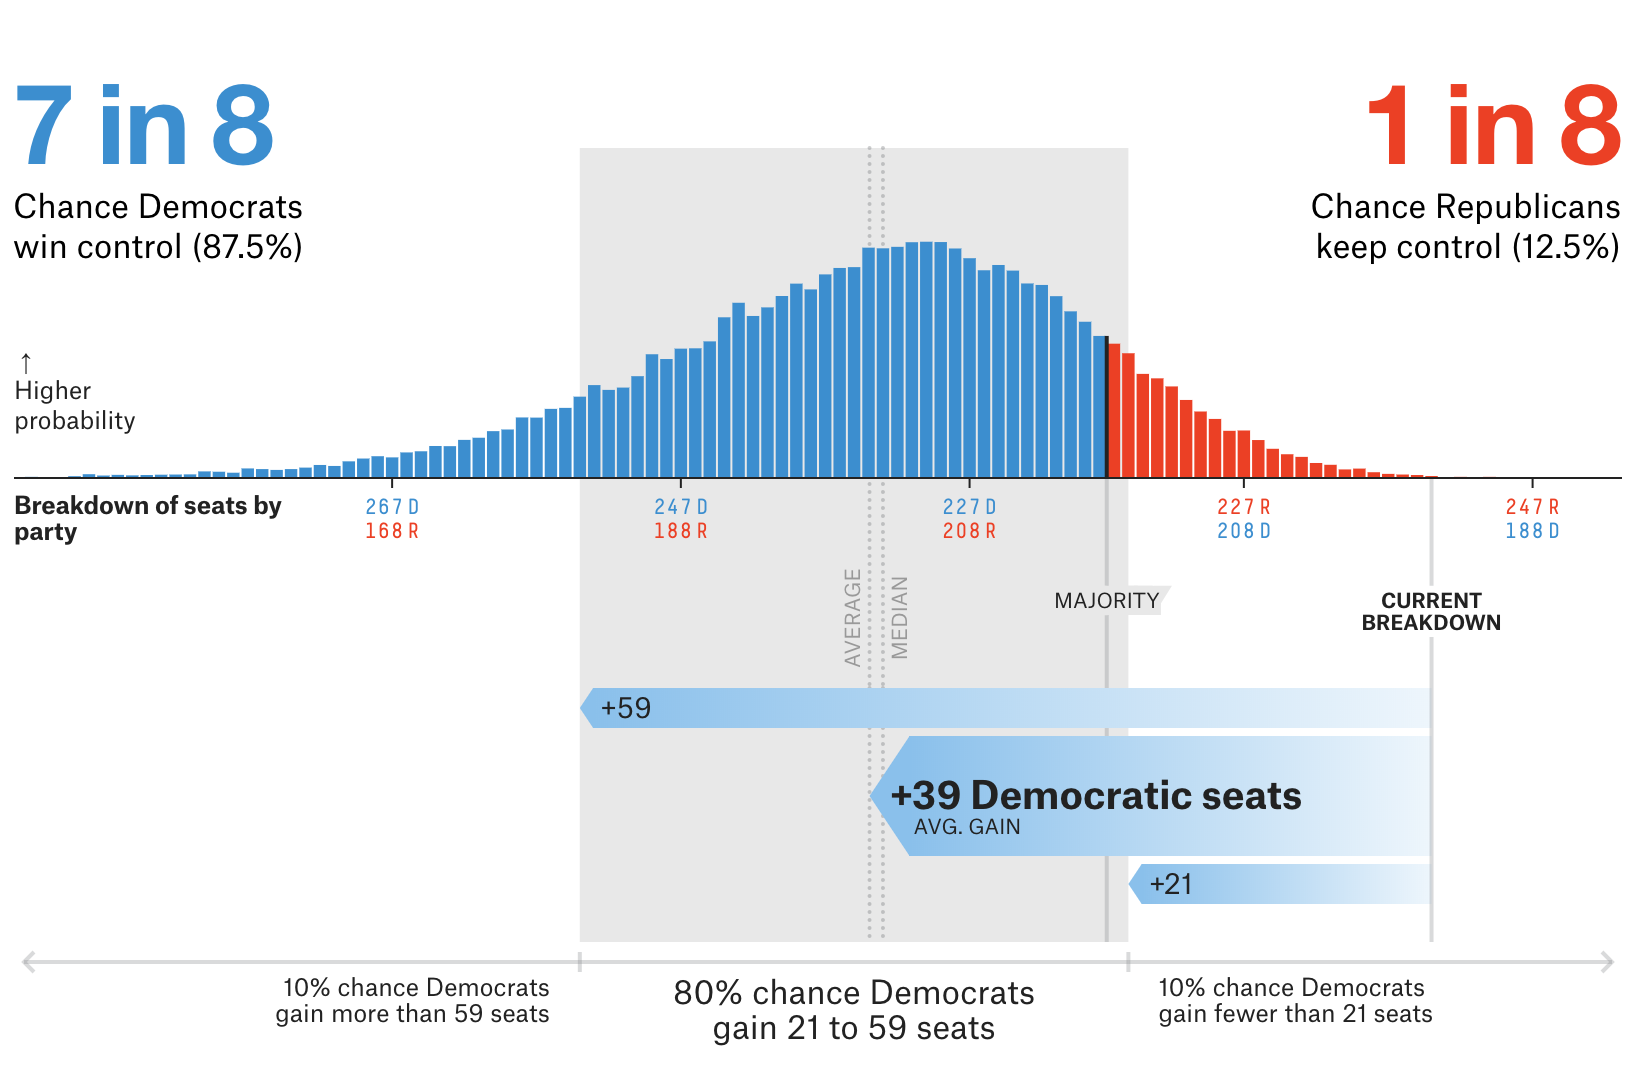
\includegraphics[scale=0.4]{538_hist}
  \caption{FiveThirtyEight Forecast for House on Nov. 5, 2018}
  \label{fig:538_hist}
\end{figure}

\begin{figure}[tbh]
  \centering
  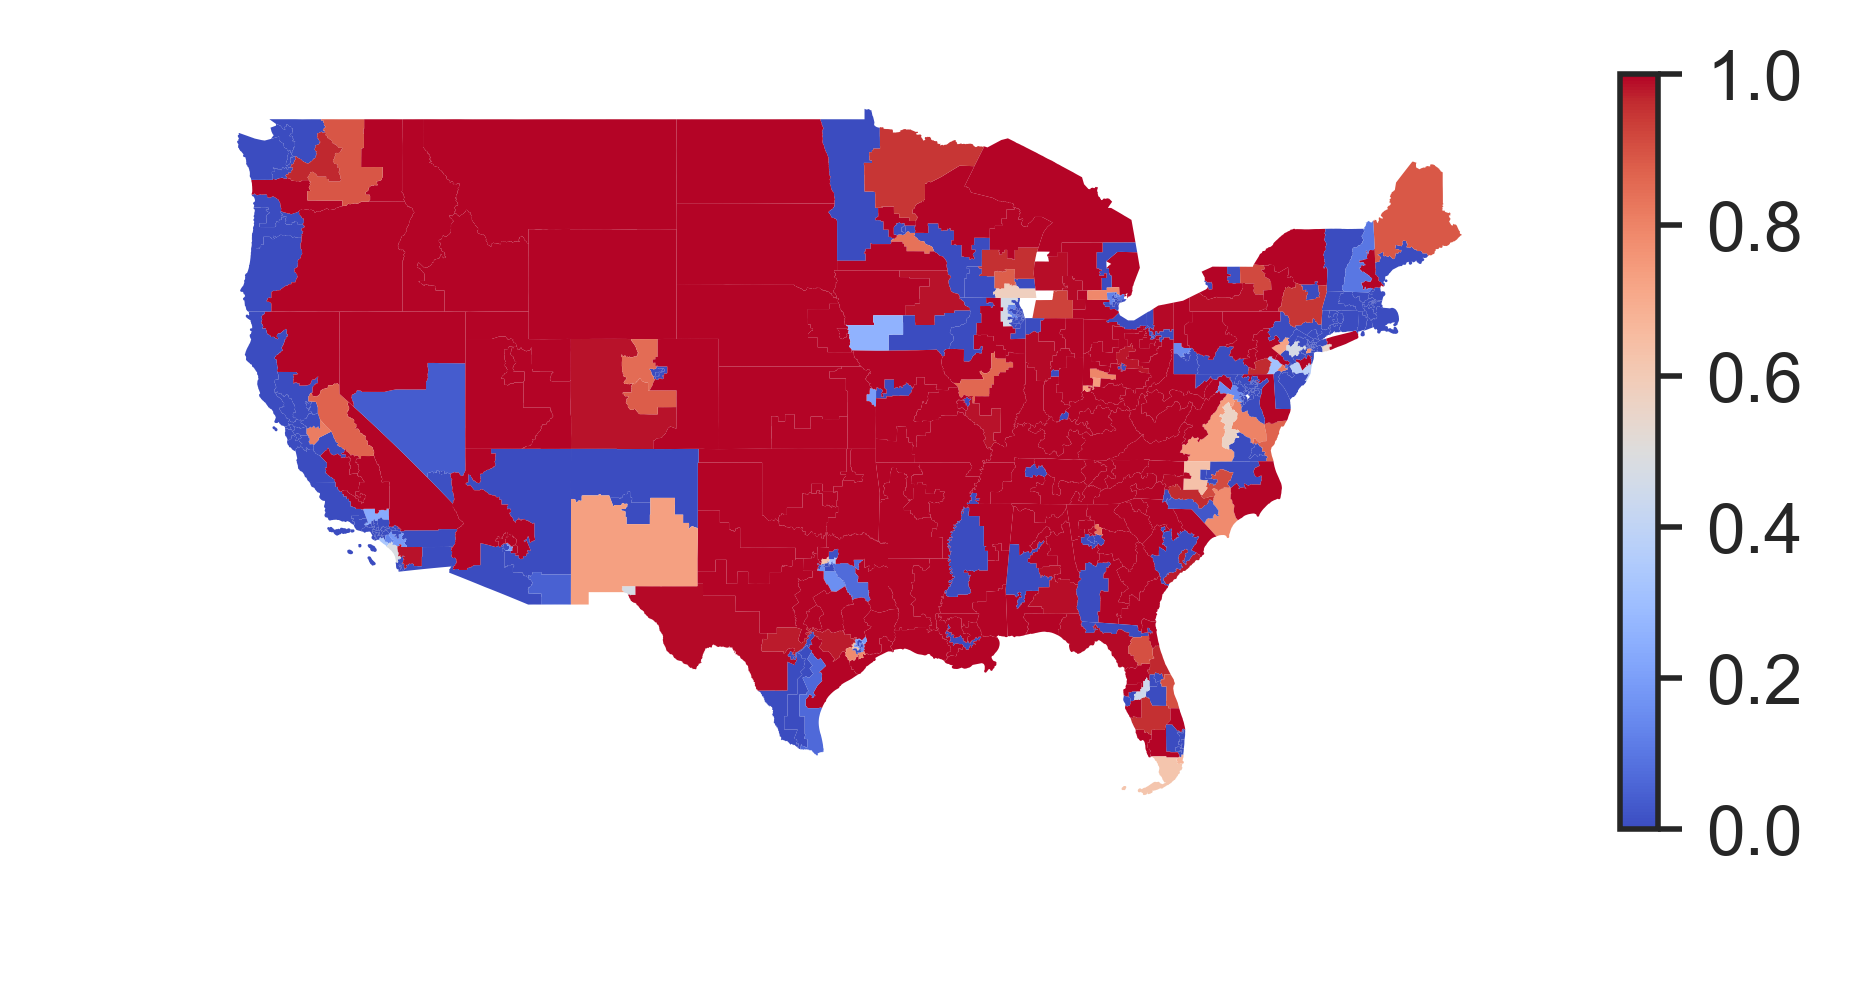
\includegraphics[scale=1.7]{projected_map.png}
  \caption{Projected marginal probabilities of Republican victory}
  \label{fig:proj_map}
\end{figure}

\begin{figure}[tbh]
  \centering
  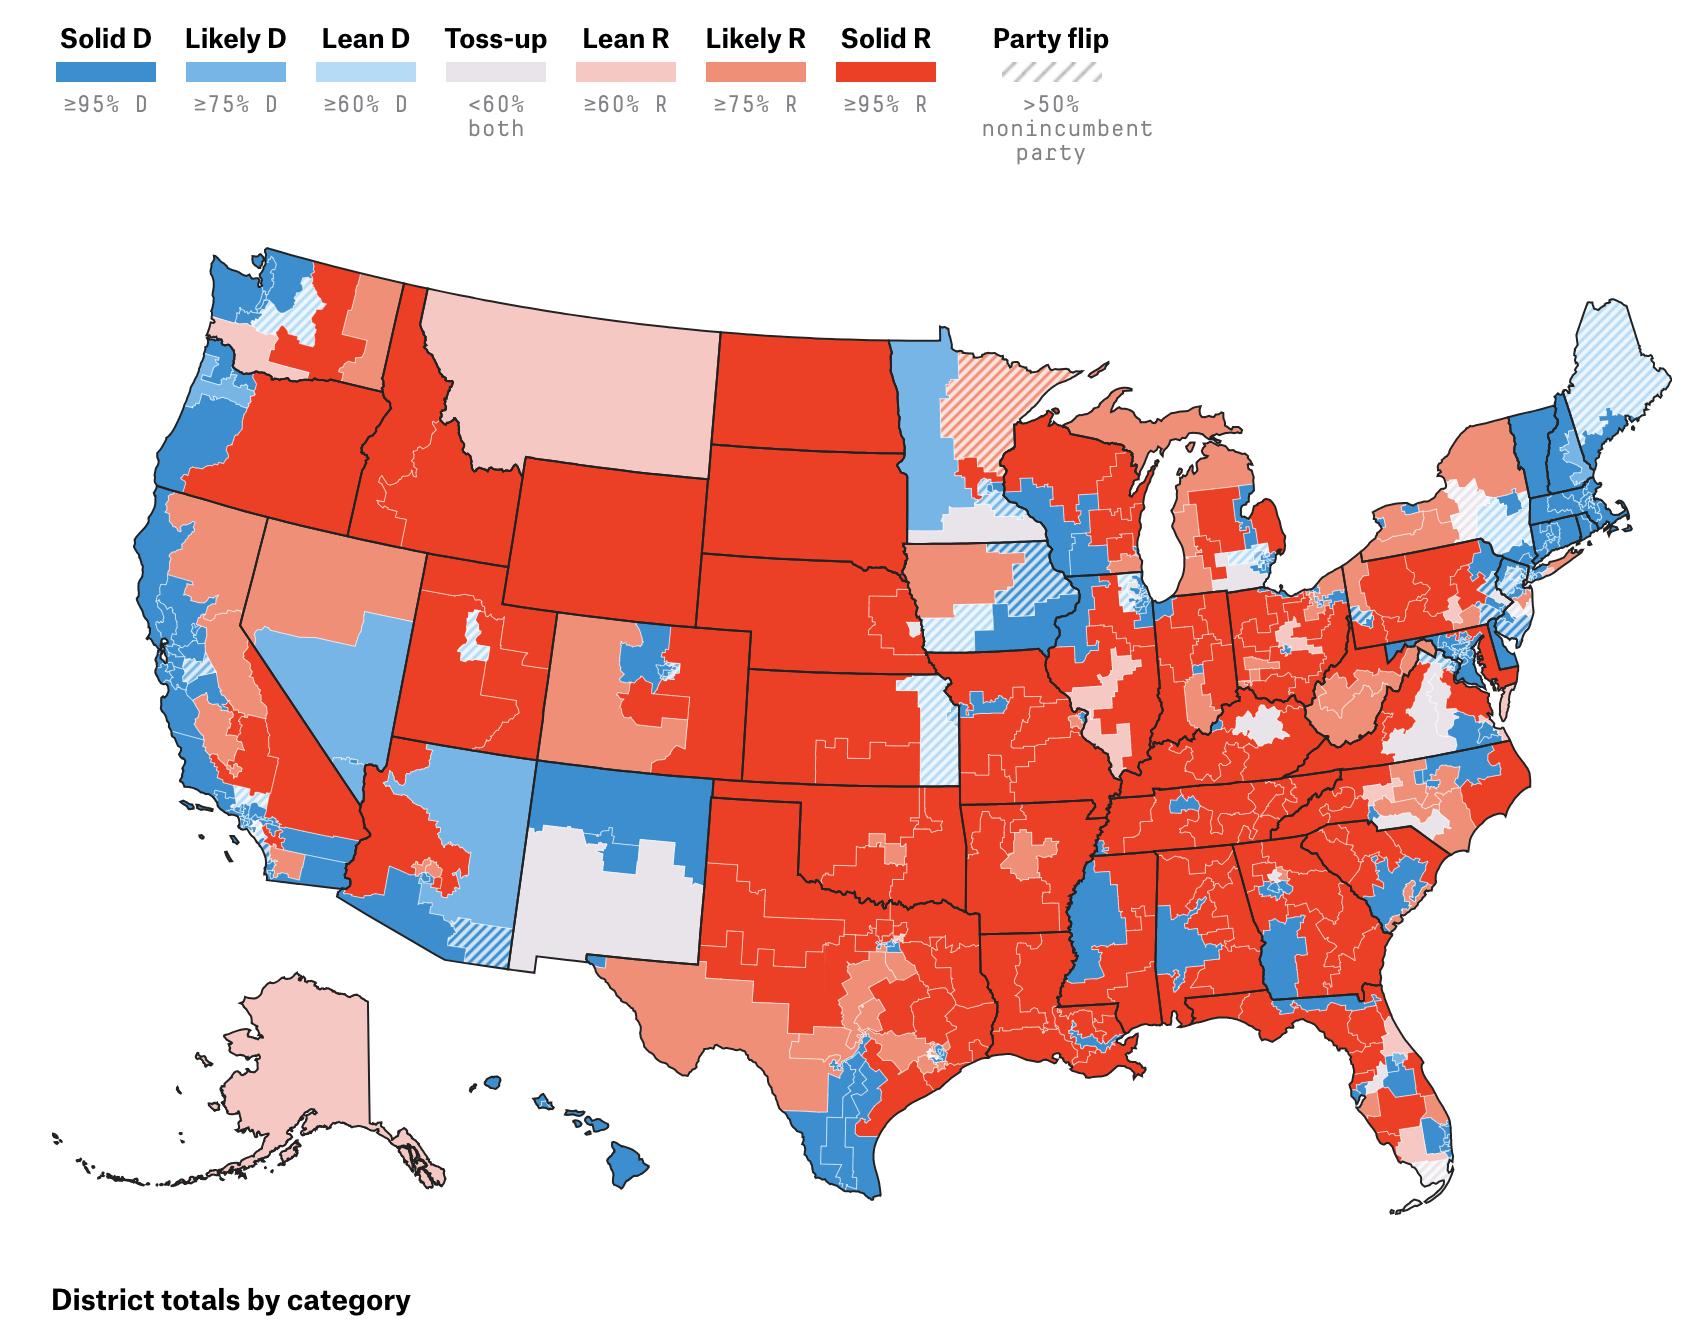
\includegraphics[scale=0.45]{538_map}
  \caption{District-level forecast by FiveThirtyEight}
  \label{fig:538_map}
\end{figure}

\bibliographystyle{jpe}
\bibliography{main.bib}

\end{document}
